\chapter{Solution} \label{solution}

The solution proposed in this thesis uses an approach where the distributed application is bundled with an encrypted ML model. To be able to decrypt the encrypted ML model, the distributed application opens a secure channel to the special, remote attestation capable key server. After the key server has validated that the application runs in a secure and isolated environment -- an enclave, and the application has not been tampered with, the key server transfers the decryption key to the application. The encrypted ML model is then decrypted inside an enclave and only used within the enclave, and never exposed outside the enclave.

Using this approach, the confidentiality and integrity of the ML application is not compromised, and the intellectual property associated with the ML model is safe. The solution proposed in this thesis is demonstrated by implementation described in the next section.

By providing a practical solution to the concern regarding the safety of the IP associated with ML models, this chapter answers to the \ref{rq2}. Later in this chapter, in Section \ref{perfandlimitations}, the issues, limitations and effects on performance are discussed, thus answering to the \ref{rq3}.

\section{Implementation} \label{implementation}

The example implementation consists of three parts; the model trainer, the key server and the distributed application itself, called predictor, which will be discussed in detail later. The model trainer trains the ML model and exports it to an encrypted file with a decryption key. The key server acts as a remote attestation capable key server from which the predictor can request a decryption key. The predictor part is the application that can be distributed to the clients. In this implementation example, the predictor is an application that predicts car fuel consumption based on user inputted details.

The predictor is bundled with an encrypted machine learning model and Gramine Python application, which runs inside Intel SGX enclave. The Gramine application has a machine learning framework bundled and utilities to request remote attestation and decryption key from the key server through a secure channel. The key server uses Intel SGX Remote Attestation to validate the enclave before providing the decryption key. Because of the key exchange and remote attestation, minimal internet connection is required in the production environment. The high-level application flow can be seen in Figure \ref{fig:sgx-flow}.

The predictor part is further divided into two parts, trusted (\textit{trusted.py}) and untrusted (\textit{predictor.py}). The trusted part (Gramine application) runs inside the Intel SGX enclave and has only the minimal needed functionality in addition to the Intel SGX related functionality. Additional capabilities are the capability to decrypt the ML model and the capability to run ML calculations on that model. The untrusted part has all the other application logic and calls the trusted part only when it is needed to do ML calculations.

\begin{figure}
\centering 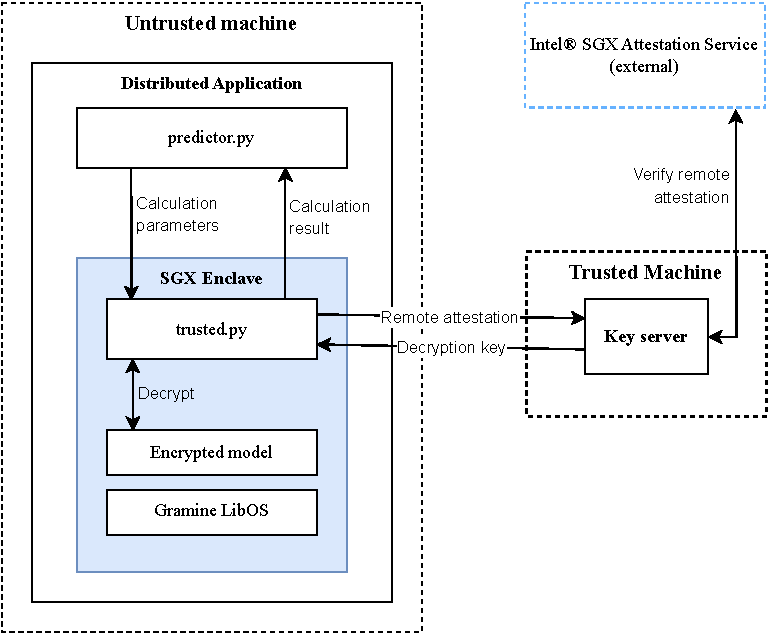
\includegraphics[width=0.8\textwidth]{img/sgx}
\caption{Application flow diagram}
\label{fig:sgx-flow}
\end{figure}

 Python was chosen as the main implementation language as Python has great machine learning tool support. Intel SGX was chosen as Trusted Execution Environment implementation. Running Python inside the SGX enclave is possible using the library operating system Gramine.\cite{gramine} Running Python inside the enclave is already demonstrated by Denghui Zhang, Guosai Wang, Wei Xu and Kevin Gao in their paper \textit{SGXPy: Protecting Integrity of Python Applications with Intel SGX}\cite{sgxpy}.

The model trainer and the key server are intended to run on the trusted infrastructure and do not require hardware Intel SGX support. Both model trainer and key server are needed to build artifacts for the distributed application. Artifacts includes key server certificate generated when the key server is built and the encrypted ML model generated by the model trainer. Furthermore, the key server needs access to the decryption key generated by the model trainer. The predictor which uses the ML model for computation is run in an untrusted environment. 

As the ML model is bundled encrypted with the predictor application and only processed decrypted inside the Intel SGX enclave, the Intellectual Property of the model owner is safe.

There is a repository containing all the software source code at GitHub\cite{githubrepo}.

\subsection{Description of the Data} \label{data}

The dataset used to train the machine learning model contains 398 instances of cars with 8 attributes. The attributes are miles per gallon (MPG), cylinders, engine displacement in cubical inches, horsepower, weight in pounds, acceleration ($ft/s^2$), year of making, origin and name of the model. Origin is marked as an integer, where 1 means United States, 2 means Europe and 3 means Japan.

The dataset is from the Machine Learning Repository by University of California, Irvine\cite{dataset}. The data is in CSV format. Example data points can be seen in Table \ref{tab:data}.

\begin{table}
\centering{}\caption{Example data points of the dataset.\label{tab:data}}
\begin{tabular}{|c|c|c|c|c|c|c|c|c|}
mpg & cyl. & displ. & hp & weight & accel. & year & origin & name \tabularnewline
\hline 
23.7 & 3 & 70.00 & 100.0 & 2420 & 12.5 & 80 & 3 & Mazda RX-7 \tabularnewline
19.0 & 6 & 156.0 & 108.0 & 2930 & 15.5 & 76 & 3 & Toyota Mark II \tabularnewline
11.0 & 8 & 400.0 & 150.0 & 4997 & 14.0 & 73 & 1 & Chevrolet Impala \tabularnewline
\end{tabular}
\end{table}

\subsection{Overview of the Application Stack} \label{overview}

\subsubsection{Model Trainer} \label{modeltrainer}

The model trainer is part of the implementation that is responsible for training the machine learning model and exporting it as an encrypted file with a decryption key. The model trainer is meant to run in a trusted environment as a part of the build process.

The original dataset needed to be cleaned for empty values and inconsistent formatting. The dataset was split into two datasets, \textit{cars1.csv} which has 242 data points (16 KB) and \textit{cars2.csv} which has 150 data points (8 KB). The \textit{cars1.csv} was used to train the model and \textit{cars2.csv} was used to test the model. Except for the car model name, all other data attributes were used to train the model.
 
As a machine learning library, the Python library \textit{Scikit-learn}\cite{scikit} was used. Linear Regression is used as an ML algorithm to train the model. Other Python libraries used were \textit{Cryptography} for cryptographic functions and \textit{Pandas} for easy CSV handling.

As the original dataset has only 398 data points, a synthetic data generator was also implemented as a part of the model trainer. Synthetic data is used in later sections to run performance testing on large datasets.

Model trainer is used in the application build process, where the model is trained, encrypted and exported to the application bundle and the decryption key is exported to the key server. The exported model is 4 KB in size.

\subsubsection{Key Server} \label{keyserver}

The key server is used to securely provide the decryption key for the predictor application. The security of the decryption key transfer is confirmed by Intel's Remote Attestation. Remote attestation confirms that the application code is running inside an enclave and the application is not tampered with. Using remote attestation makes sure that the decryption key (and decrypted ML model) is only handled inside an enclave, and it is impossible for the application user to obtain the key or the decrypted model. The key server is meant to run in a trusted environment.

The key server is a C application based on Intel's example code. The key server acts as an HTTPS server from which the application can request the decryption key. When the application requests for the key, the Remote Attestation is performed and if it is successful, the key server returns the decryption key.

\subsubsection{Predictor} \label{predictor}

The predictor application is the main application which is meant to be distributed to the end user and run inside an untrusted environment. The application predicts fuel consumption of a car based on the car's other attributes that are inputted by the end user. There are also options for running the predictions for a predefined dataset or running predictions locally, outside the Intel SGX enclave. These additional options are mainly for performance testing purposes.

The predictor application follows Intel SGX application structure and has two parts; untrusted and trusted. The untrusted part (\textit{implementation/predictor/predictor.py} in the GitHub repository) has all the application logic and calls the trusted part only for the ML calculations. Executing the untrusted part starts the predictor application and is meant to be called directly by the end user. Trusted part (\textit{implementation/predictor/trusted/trusted.py} in the GitHub repository) is the part of the application that is responsible for handling all the sensitive tasks. Sensitive tasks are the handling of the decryption key and decrypted ML model.

An encrypted machine learning model is bundled with the predictor application. Model is handled in plain only inside the trusted part, and it is impossible to decrypt it outside the trusted part.

When the application is started by invoking the untrusted part, it asks the user for the car details. After the details are filled in, the trusted part is invoked by the untrusted part and the car details are sent to the trusted part.

When the trusted part is invoked, the Intel SGX enclave is created and initialized, remote attestation is requested from the key server, and after successful remote attestation, the decryption key is received from the key server. Now the encrypted ML model that is bundled with the application is decrypted, and the ML calculations are performed, all inside the trusted part.

After the ML calculations are ready, the results returned to the untrusted part, which formats them and presents to the user. Results include the predicted fuel consumption, running time, data point count and, in a case of running predictions on a dataset, the R2 score, which is a calculated metric describing the accuracy of the ML model.

The application has a simple command line interface for interacting with the user. Trusted and untrusted part communicate with each other with a simple interface, which was implemented. The interface for inter-application communication used command line parameters to send data to the trusted part and standard output to receive results from the trusted part. The data format is JSON. An example of the communication between the untrusted and the trusted part can be seen in Listing \ref{alg:communication}.

In a production-ready application, the inter-application communication interface should be more sophisticated. For example, running an HTTP server inside an enclave is possible.

\begin{algorithm}
\begin{minted}{python}
# To trusted part
{'cylinders': [4], 'displacement': [97.5], 'horsepower': [114.0],
'weight': [2094], 'acceleration': [10.5], 'year': [90], 'origin': [3]}

# From trusted part
{'predictions': [39.557013442440216], 'time': 0.004551887512207031,
'count': 1, 'r2': null}
\end{minted}
\caption{An example of inter-application communication.\label{alg:communication}}
\end{algorithm}

\subsection{Setting Up} \label{settingup}

Next, the requirements and prerequisites which are needed to build the application and the build of the application are discussed in detail.

\subsubsection{Requirements} \label{requirements}

The model trainer can be run anywhere where there is Python available and enough resources to train a simple machine learning model.

The key server needs working Gramine installation with remote attestation support. Hardware Intel SGX support is not needed.

The predictor application needs an environment that supports Intel SGX. Section \ref{usingsgxonlinux} and \textit{Intel® SGX Software Installation Guide For Linux* OS}\cite{sgxinstall} can be referred for detailed instructions. Gramine documentation\cite{graminedocs} can be referred for Gramine installation instructions.

The next Python libraries need to be installed system-wide. The easiest way is to install them is to install them from the distribution package repositories.

\begin{itemize}
  \item \textit{scikit-learn} as a machine learning framework.
  \item \textit{cryptography} for cryptographic functions.
  \item \textit{pandas} for handling CSV's.
  \item \textit{joblib} for exporting and importing ML models.
\end{itemize}

\subsubsection{Remote Attestation} \label{remoteatt}

The implementation uses the \textit{Intel SGX Attestation Service Utilizing Enhanced Privacy ID (EPID)} method for remote attestation. Developer access for Intel EPID can be requested from the Intel Trusted Services Portal.\cite{intelportal} This implementation requires unlinkable EPID subscription, which is free for non-commercial use.

The SPID identifier and EPID API key can be acquired from Intel Trusted Services Portal after subscription.

\subsubsection{Build} \label{build}

After the Intel SGX support, Gramine and other dependencies are installed, the application itself can be built. The application code can be downloaded from \url{https://github.com/mjturt/thesis}. In the application's implementation folder, the example settings file \textit{settings.sh-example} needs to be copied to \textit{settings.sh}. At least two configuration parameters need to be configured in the settings file. Configuration parameters \mintinline{bash}{RA_CLIENT_SPID} and \mintinline{bash}{RA_TLS_EPID_API_KEY} represents SPID identifier and EPID API key, which were obtained from Intel Trusted Services Portal in the last section.

In the implementation folder, there is a \textit{build.sh} script to automate the build process. The build script initiates the model trainer, which trains the ML model with data from file \textit{implementation/model-trainer/data/cars1.csv}. When the model is trained, the model trainer encrypts it and exports the encrypted model and the decryption key to files. The build script then makes the encrypted model available to the predictor and the decryption key available to the key server. After that, the key server is compiled and built. The key server exports the needed SSL certificate as a part of the build process, and the build script makes it available to the predictor.

Next, the build script instructs the user how the predictor can be built and how to launch the application. When the predictor is built based on these instructions, the application stack can be launched, which will be covered in the next section. An example installation process can be seen in Listing \ref{alg:install} and a diagram of the build flow can be seen in Figure \ref{fig:sgx-build}.

\begin{figure}
\centering 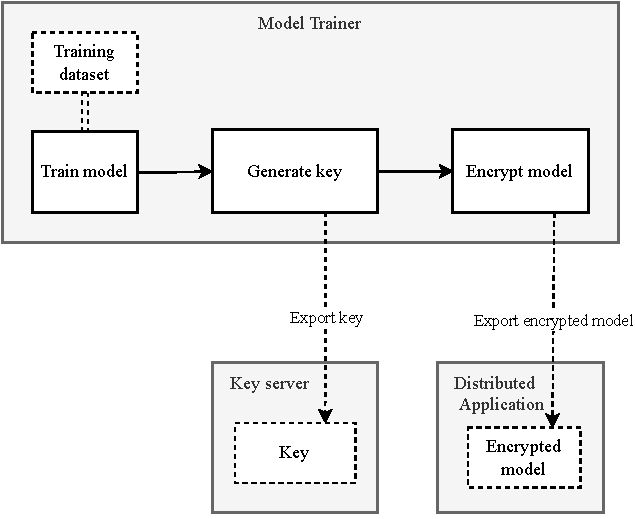
\includegraphics[width=0.8\textwidth]{img/sgx_build}
\caption{Build flow}
\label{fig:sgx-build}
\end{figure}

In a real-life scenario, the predictor could now be packed and distributed to the end-users, but for simplicity, the whole application stack is run on the same machine.

\begin{algorithm}
\begin{minted}{bash}
git clone https://github.com/mjturt/thesis.git
cd thesis/implementation
cp settings.sh-example settings.sh  # and configure
source settings.sh
./build.sh
cd predictor/trusted
make SGX=1
\end{minted}
\caption{Installation procedure of the application.\label{alg:install}}
\end{algorithm}

\subsection{Usage} \label{usage}

After installation is complete, the key server can be started in the \textit{implementation/key-server} folder by running \mintinline{bash}{./server_epid}. The key server is left running. Now the setting up is complete, another shell session needs to be opened, and then the predictor can be executed in the \textit{implementation/predictor} folder by running \mintinline{bash}{python predictor.py}. The settings file \textit{settings.sh} must always be sourced in the shell session from where the key server or predictor is invoked.

\begin{algorithm}
\begin{minted}{text}
...
For a car:

Model: Mazda MX-5
Cylinders: 4
Displacement: 97.5 in³ (1597.7 cm³)
Power: 114.0 hp (85.0 kW)
Weight: 2094.0 lb (950.0 kg)
Acceleration: 10.5 ft/s² (3.2 m/s²)
Year: 1990
Origin: Japan
Predicted consumption: 39.6 mpg (5.9 l/100km)

The predicted consumption is 5.9 l/100km
The prediction calculation took 0.004552 seconds
\end{minted}
\caption{Output of the predictor application without any parameters.\label{alg:output}}
\end{algorithm}

\begin{algorithm}
\begin{minted}{text}
Sending dataset cars.csv to the Gramine Intel SGX enclave for
calculation...

--- START OF GRAMINE OUTPUT ---
...
--- END OF GRAMINE OUTPUT ---

Consumption prediction calculation for 150 car instances took
0.002998 seconds
R2 score: 0.81
\end{minted}
\caption{Output of the predictor application using a dataset.\label{alg:output2}}
\end{algorithm}

Without any parameters, the predictor application \textit{predictor.py} asks the user for the car details and then runs ML calculations inside an enclave. The predictor can be invoked with a command line argument \mintinline{bash}{--help} to get all available command line argument options. Available command line arguments include an argument to run predictions on a predefined dataset and an argument to disable Intel SGX. An example output of the predictor without any parameters and after it has asked the car details can be seen in Listing \ref{alg:output}. Non-relevant output has been omitted.

An example output of the predictor using a predefined dataset can be seen in Listing \ref{alg:output2}. In this listing, only the Gramine output is omitted.

\section{Performance and Limitations} \label{perfandlimitations}

In this section, the testing setup used to conduct performance testing is described, including the hardware and software used. The performance testing research setting is described, and the performance testing results are then presented, and perceived limitations and downsides are discussed. The general limitations of Intel SGX can be read from Section \ref{limitations}.

\subsection{Testing Setup} \label{setup}

For the simplicity sake, in the testing setup, the model trainer, the key server and the distributed app are built and run on the same machine.

As a testing hardware, Dell Latitude 5490 laptop provided by the University is used. The laptop has an 8th generation Intel Core i5 processor that has Intel SGX support. The specifications of the testing hardware and software below:

\begin{itemize}
  \item \textbf{OS:} Ubuntu Server 22.10 
  \item \textbf{Kernel:} Linux 5.10.15
  \item \textbf{CPU:} Intel Core i5-8350U 8-core 3.6 GHz (code name Kaby Lake R)
  \item \textbf{Memory:} 16 GB
\end{itemize}

The processor did not have Flexible Launch Control (Intel SGX Launch Control) support, so the Linux in-kernel SGX driver could not be used, as the in-kernel driver requires it. Out-of-tree (OOT) driver was used instead.

As an operating system, Ubuntu Linux 22.10 was used. As of the time of writing, Ubuntu 22.10 used kernel version 5.19 that has the in-kernel SGX driver that is incompatible with the out-of-tree SGX driver. The Linux kernel version had to be downgraded to version 5.10.

After downgrading the kernel, the Intel's official documentation\cite{sgxinstall} to install out-of-tree SGX driver was followed.

Next, the Gramine library OS can be installed. Because of the OOT driver, Gramine needed to be built from source. Gramine documentation\cite{graminedocs} was followed to build Gramine from source with custom options.

All needed Python libraries were installed system-wide from the default Ubuntu APT repositories.

As the processor model is older than the Ice Lake series, the EPC size is limited to 98 MB. With enclaves that require more than that, there would be substantial performance degradation. As the Intel SGX OOT driver does not support EPC swapping, testing with enclaves larger than 98 MB could not be performed.

\subsection{Performance} \label{performance}

As Machine Learning calculations can be expensive, the overhead produced by running the calculations inside the Intel SGX enclave must be carefully considered. The usability of this solution depends on how much Intel SGX adds overhead.

In the testing setup, a dataset with 150 data points and a dataset with one million data points representing cars were used. The dataset with 150 data points was from the original dataset (file \textit{implementation/model-trainer/data/cars2.csv} in the repository), and the dataset with one million data points was generated with the model trainer's data generation utility. Running inference for data points ran as a batch and total time was recorded. The predictor application has an option to run inference inside Intel SGX enclave or locally. The two methods to run inference are then compared.

\begin{algorithm}
\begin{minted}{python}
test_X, test_y = build_data(data)
start = time()
result = model.predict(test_X)
end = time()
elapsed_time = end - start
\end{minted}
\caption{Python code to run inference and measure time elapsed.\label{alg:time}}
\end{algorithm}

Only the run time of the actual inference is recorded, as can be seen in Listing \ref{alg:time}. Other performance implications to the process are reviewed separately.

For both methods and both datasets, 5 runs conducted and then an average of running time is calculated. Running times for 150 data point inference can be seen in Table \ref{tab:performance} and running times for one million data point inference can be seen in Table \ref{tab:performance2}.

The dataset with 150 data points was 4 KB in size and the dataset with one million data points was 44 MB in size, so the EPC size limit did not affect the measurements.

Based on performance testing, running inference inside the Intel SGX enclave is considerably slower than without the Intel SGX enclave, based on the dataset size. With the smaller dataset, the inference inside SGX enclave is only approximately two times slower, but when a dataset grows to one million data points, the inference inside SGX enclave is approximately thirty-three times slower. It seems that the bigger the dataset is, the more the Intel SGX is lowering the performance.

\begin{table}
\centering{}\caption{Run times of 150 data point inference with both methods.\label{tab:performance}}
\begin{tabular}{|c|c|c|}
Run & Intel SGX & Local \tabularnewline
\hline 
1 & 2.75 ms & 0.97 ms \tabularnewline
2 & 3.01 ms & 0.99 ms \tabularnewline
3 & 2.73 ms & 0.96 ms \tabularnewline
4 & 3.05 ms & 0.99 ms \tabularnewline
5 & 3.20 ms & 0.97 ms \tabularnewline
\hline 
\textbf{Average} & \textbf{2.95 ms} & \textbf{0.98 ms} \tabularnewline
\end{tabular}
\end{table}

\begin{table}
\centering{}\caption{Run times of million data point inference with both methods.\label{tab:performance2}}
\begin{tabular}{|c|c|c|}
Run & Intel SGX & Local \tabularnewline
\hline 
1 & 782.19 ms & 23.15 ms \tabularnewline
2 & 784.03 ms & 23.35 ms \tabularnewline
3 & 787.77 ms & 24.04 ms \tabularnewline
4 & 791.85 ms & 23.19 ms \tabularnewline
5 & 792.61 ms & 23.88 ms \tabularnewline
\hline 
\textbf{Average} & \textbf{787.69 ms} & \textbf{23.52 ms} \tabularnewline
\end{tabular}
\end{table}

Besides the actual running time, the initialization of the Intel SGX application needs to be considered. Initialization of the Gramine, the enclave and performing Remote Attestation takes up to one minute on the testing machine. In the testing setup, the application and the key server run on the same machine, so network latency can increase the initialization in production environment. In any case, the Intel SGX application is usually kept running and initialization does not happen every time when interacting with the application.

\subsection{Limitations and Drawbacks} \label{perceivedlimitations}

One of the most obvious limitations is the EPC size limit of 98 MB in the testing setup. On the testing machine, it is impossible to run enclaves bigger than the EPC size. When tried to run inference for a dataset with 3 million data points (130 MB), the application simply fails because not enough memory could be allocated. However, the EPC size limit is an issue only with older Intel hardware.

In a scenario where the ML application is distributed to the end-users, the hardware and software requirements that end-users must meet, might become a major limitation. End-users infrastructure must fully support Intel SGX, which may make this solution unappealing to some potential customers. One possible solution to this problem is that the ML application is provided as an end-to-end solution, where infrastructure and support is included in the product. This obviously increases the cost of the solution.

The major downside of the approach of using Intel SGX to protect ML models is the engineering overhead it adds. Hardware and software must be carefully chosen, so that the full potential of Intel SGX can be reached. Configuring the system to fully support Intel SGX is a complex operation which requires understanding of the hardware and operating system used. Building Intel SGX applications is more complex than building just regular applications, though frameworks like Gramine can help the process.
